\section{Pyramidal Dice}
The final shape that we explored was the pyramidal dice. We have a base with either four or five vertices on the same plane (depending on whether we want a five or six sided pyramid) and a vertex above this plane with all non-base faces being triangles.\\
\begin{figure}[h]
\center
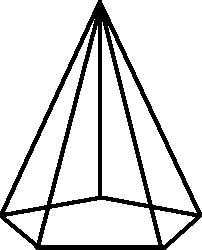
\includegraphics[scale=1]{p-pyramid.png}
\caption{Pentagonal Pyramid with six sides}
\label{fig:pent_p}
\end{figure}

\begin{figure}[h]
\center
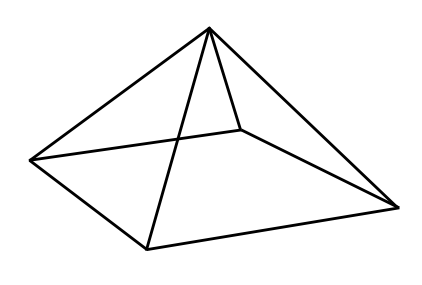
\includegraphics[scale=1]{pyramid_height.png}
\caption{Square Pyramid with five sides}
\label{fig:square_p}
\end{figure}

There were two main reasons for choosing this particular shape:\\
\begin{itemize}
    \item We needed one face with a probability close to half, and the base of a pyramid would be an elegant way to do this.\\
    \item This shape exists for both six and five sided dice, making it easy to extend our simulator and analysis to work for both types.\\
\end{itemize}

\subsection{Optimization Algorithms}
We modelled the pyramidal shape as follows:\\
\begin{itemize}
    \item A height h, denoting the vertical height of the topmost point from the plane containing the base.\\
    \item The origin of our coordinate system is the point vertically below the topmost point lying on the base plane.\\
    \item The first point, which lies on the x axis (which we define arbitrarily)
\end{itemize}
